\documentclass[polish,polish,a4paper]{article}
\usepackage[polish]{babel}
\usepackage[T1]{fontenc}
\usepackage[utf8]{inputenc}
\usepackage{pslatex}
\usepackage{pgfplots}
\usepackage{circuitikz} 
\usepackage{setspace}
\usepackage{caption}
\usepackage{amssymb}
\usepackage{amsmath}
%\usetikzlibrary{circuits.ee.IEC}
\usepackage{anysize}
\usepackage{graphicx}
\usepackage{hyperref}
\usepackage{float}
\hypersetup{
	colorlinks=true,
	linkcolor=blue,
	filecolor=magenta,      
	urlcolor=cyan,
}

\marginsize{2.5cm}{2.5cm}{2cm}{2cm}

\newcommand{\PRzFieldDsc}[1]{\sffamily\bfseries\scriptsize #1}
\newcommand{\PRzFieldCnt}[1]{\textit{#1}}
\newcommand{\PRzHeading}[8]{
	%% #1 - nazwa laboratorium
	%% #2 - kierunek 
	%% #3 - specjalność 
	%% #4 - rok studiów 
	%% #5 - symbol grupy lab.
	%% #6 - temat 
	%% #7 - numer lab.
	%% #8 - skład grupy ćwiczeniowej
	
	\begin{center}
		\begin{tabular}{ p{0.32\textwidth} p{0.15\textwidth} p{0.15\textwidth} p{0.12\textwidth} p{0.12\textwidth} }
			
			&   &   &   &   \\
			\hline
			\multicolumn{5}{|c|}{}\\[-1ex]
			\multicolumn{5}{|c|}{{\LARGE #1}}\\
			\multicolumn{5}{|c|}{}\\[-1ex]
			
			\hline
			\multicolumn{1}{|l|}{\PRzFieldDsc{Kierunek}}	& \multicolumn{1}{|l|}{\PRzFieldDsc{Specjalność}}	& \multicolumn{1}{|l|}{\PRzFieldDsc{Rok studiów}}	& \multicolumn{2}{|l|}{\PRzFieldDsc{Symbol grupy lab.}} \\
			\multicolumn{1}{|c|}{\PRzFieldCnt{#2}}		& \multicolumn{1}{|c|}{\PRzFieldCnt{#3}}		& \multicolumn{1}{|c|}{\PRzFieldCnt{#4}}		& \multicolumn{2}{|c|}{\PRzFieldCnt{#5}} \\
			
			\hline
			\multicolumn{4}{|l|}{\PRzFieldDsc{Temat Laboratorium}}		& \multicolumn{1}{|l|}{\PRzFieldDsc{Numer lab.}} \\
			\multicolumn{4}{|c|}{\PRzFieldCnt{#6}}				& \multicolumn{1}{|c|}{\PRzFieldCnt{#7}} \\
			
			\hline
			\multicolumn{5}{|l|}{\PRzFieldDsc{Skład grupy ćwiczeniowej oraz numery indeksów}}\\
			\multicolumn{5}{|c|}{\PRzFieldCnt{#8}}\\
			
			\hline
			\multicolumn{3}{|l|}{\PRzFieldDsc{Uwagi}}	& \multicolumn{2}{|l|}{\PRzFieldDsc{Ocena}} \\
			\multicolumn{3}{|c|}{\PRzFieldCnt{\ }}		& \multicolumn{2}{|c|}{\PRzFieldCnt{\ }} \\
			
			\hline
		\end{tabular}
	\end{center}
}



\begin{document}


	\PRzHeading{Laboratorium Podstaw Elektroniki}{Informatyka}{--}{I}{I3}{Układy Diodowe}{4}{Piotr Więtczak(132339), Robert Ciemny(136693), Kamil Basiukajc(136681)}

	\section{Charakterystyka stałoprądowa dla diody złączowej}
	
	\subsection{Cel zadania}
	
	Zbadanie charakterystyki stałoprądowej dla diody złączeniowej.
	
	\subsection{Przebieg zadania}
	
	Rzeczywista wartość rezystancji rezystora $1k\Omega$ wyniosła $0.977k\Omega$.
	\subsubsection{Kierunek przewodzenia}
%%%%Obwód kierunek przewodzenia
	\begin{figure}[H]
		\begin{equation*}
		\begin{circuitikz}{american}
		\draw
		(0,0) to (6,0)
		to [esource] (6,2)
		to (4,2)
		to [european resistor, a = $R$, l = $1k\Omega$] (4,0)
		(6,1) node[anchor=mid] {V}
		(0,0) to [american voltage source, l=$U_{in}$,a = $0..5V$] (0,2)
		to [Do, l= $D_{1}$, a = $1N4007$] (4,2);
		
		\end{circuitikz}
		\end{equation*}
		\captionof{figure}{Układ do badania charakterystyki statycznej diody (Kierunek przewodzenia)}
	\end{figure}

	%Tabela 
	\begin{spacing}{1.5}
		\begin{equation*}
		\begin{array}{|r|r|r|r|}
		\hline
		U_{in}\quad[V]&U_{R}\quad[V]&U_{D} = U_{in} - U_{R}\quad[V]&I_{D} = \dfrac{U_{R}}{R}\quad[mA]\\\hline
0.5&0.102&0.398&0.104\\
1&0.553&0.447&0.566\\
1.5&1.017&0.483&1.041\\
2&1.551&0.449&1.588\\
2.5&2.063&0.437&2.112\\
3&2.495&0.505&2.554\\
3.5&3.048&0.452&3.12\\
4&3.518&0.482&3.601\\
4.5&3.995&0.505&4.089\\
5&4.495&0.505&4.601\\
\hline
		\end{array}
		\end{equation*}
		\captionof{table}{Tablela przedstawiająca wyniki pomiarów i obliczeń dla kierunku przewodzenia}
	\end{spacing}

	\subsubsection{Kierunek zaporowy}

%%%%Obwód kierunek zaporowy
\begin{figure}[H]
	\begin{equation*}
	\begin{circuitikz}{american}
	\draw
	(0,0) to (6,0)
	to [esource] (6,2)
	to (4,2)
	to [european resistor, a = $R$, l = $1k\Omega$] (4,0)
	(6,1) node[anchor=mid] {V}
	(0,0) to [american voltage source, l=$U_{in}$,a = $0..5V$] (0,2)
	(4,2 )to [Do, a= $D_{1}$, l = $1N4007$] (0,2);
	
	\end{circuitikz}
	\end{equation*}
	\captionof{figure}{Układ do badania charakterystyki statycznej diody (Kierunek zaporowy)}
\end{figure}

	%Tabela 
\begin{spacing}{1.5}
	\begin{equation*}
	\begin{array}{|r|r|r|r|}
	\hline
	U_{in}\quad[V]&U_{R}\quad[mV]&U_{D} = U_{in} - U_{R}\quad[V]&I_{D} = \dfrac{U_{R}}{R}\quad[mA]\\\hline
	5&-0.003&5&0\\
	10&-0.001&10&0\\
	15&-0.002&15&0\\
	\hline
	\end{array}
	\end{equation*}
	\captionof{table}{Tablela przedstawiająca wyniki pomiarów i obliczeń dla kierunku zaporowego}
\end{spacing}


\subsubsection{Przebieg charakterystyki $I_{D} = f (U_{D})$ dla diody spolaryzowanej w kierunku zaporowym i przewodzenia}

	%%WYKRES I_{D}
\begin{figure}[H]
	\centering
	\begin{tikzpicture}
	\begin{axis}[
	width=0.9\textwidth,
	height = 0.5\textwidth,
	title={Przebieg charakterystyki $I_{D} = f(U_{D})$ dla diody spolaryzowanej w kierunku
		zaporowym i przewodzenia.},
	xlabel={Wartości napięcia zasilania źródła $U_{in}$ $V$},
	ylabel={Wartości prądów diody $I_{D}$ $[mA]$},
	%
	scaled x ticks = false,
	xtick distance = 0.5,
	x tick label style={/pgf/number format/fixed},
	%xticklabel style = {rotate= 90},
	x label style={at={(axis description cs:0.5,-0.15)},anchor=north},
	%%
	ytick distance = 0.5,
	scaled y ticks = false,
	y tick label style={/pgf/number format/fixed},
	y label style={at={(axis description cs:-0.05,0.85)},anchor=east},
	%%
	legend pos=north west,
	ymajorgrids=true,
	grid style=dashed,
	]
	%%
	\addplot[
	color=black,
	mark=*,
	]
	coordinates {
		(0.5,0.104)(1,0.566)(1.5,1.041)(2,1.588)(2.5,2.112)(3,2.554)(3.5,3.12)(4,3.601)(4.5,4.089)(5,4.601)
	};
	%%
	\addplot[
	color=blue,
	]
	coordinates {
(0.5,0)(1,0)(1.5,0)(2,0)(2.5,0)(3,0)(3.5,0)(4,0)(4.5,0)(5,0)
	};
	\legend{
		kierunek przewodzenia,
		kierunek zaporowy,
	}
	%%
	\end{axis}
	\end{tikzpicture}
\end{figure}


\section{Badanie prostownika jednopołówkowego}
\subsection{Cel zadania}

	Badanie prostownika jednopołówkowego.

\subsection{Przebieg zadania}

	Rzeczywista wartość rezystancji rezystora $10k\Omega$ wyniosła $9.899k\Omega$.

%%%%Bez voltomierza
\begin{figure}[H]
	\begin{equation*}
	\begin{circuitikz}{american}
	\draw
	(0,0) to (4,0)
	to [european resistor, l = $R$, a = $10k\Omega$] (4,2)
	(0,0) to [sV, l=$U_{sin}$,a = $5V$] (0,2)
	to [Do, l= $D_{1}$, a = $1N4007$] (4,2);
	\draw [red]
	(-2,2.65) node[anchor=mid] {Czerwony przewód}
	(-2,2.25) node[anchor=mid] {z kanału X oscyloskopu}
	(6,2.65) node[anchor=mid] {Czerwony przewód}
	(6,2.25) node[anchor=mid] {z kanału Y oscyloskopu}
	(0,2) to [short, *-,color = red] (-4,2)
	(4,2) to [short, *-,color = red] (8,2);
	\draw
	(0,0) to [short, *-] (-4,0)
	(4,0) to [short, *-] (8,0)
		(-2,0.65) node[anchor=mid] {Czerwony przewód}
	(-2,0.25) node[anchor=mid] {z kanału X oscyloskopu}
	(6,0.65) node[anchor=mid] {Czerwony przewód}
	(6,0.25) node[anchor=mid] {z kanału Y oscyloskopu};
	\end{circuitikz}
	\end{equation*}
	\captionof{figure}{Układ pomiarowy dla badania własności prostownika jednopołówkowego}
\end{figure}


\begin{figure}[H]
	\centering
	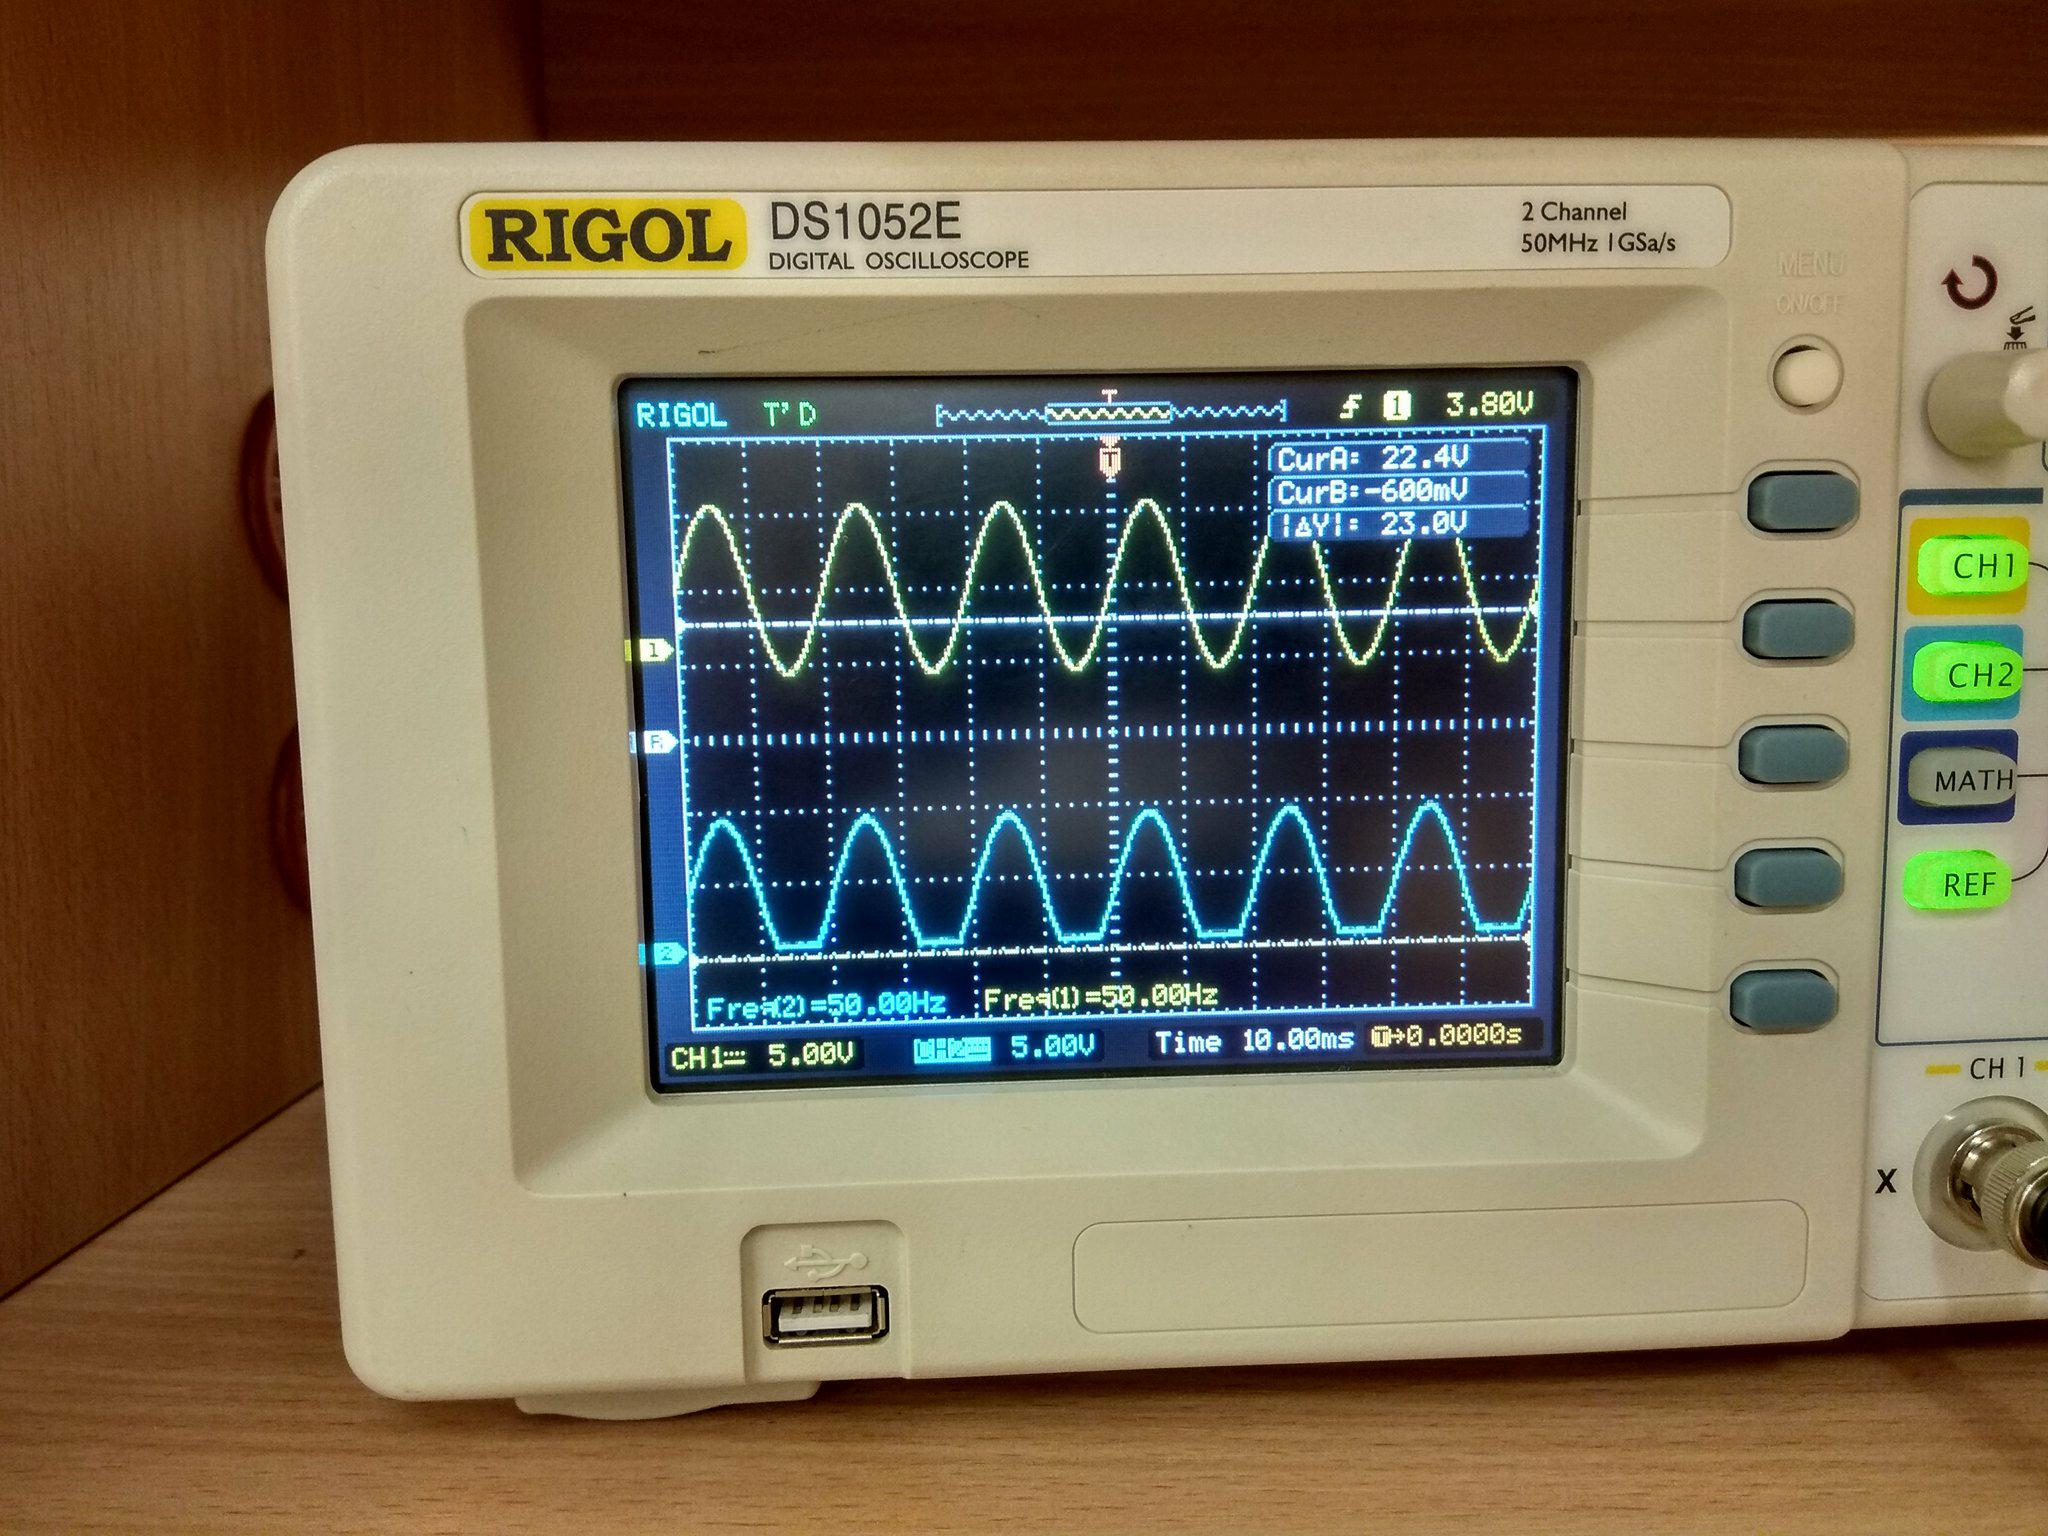
\includegraphics[scale=0.2]{1.jpg}
	\captionof{figure}{Kształat przebiegu napięcia na wejściu i wyjściu prostownika przy częstotliwości rzebiegu wejściowego równej $50Hz$}
\end{figure}

Przy częstotliwości wejściowej równej $50Hz$ amplituda napięcia przebiegu wejściowego wyniosła $1,94V$, a $1.24V$ na przebiegu wyjściowym . Różnica między przebiegiem wejściowym oraz wyjściowym wyniosła $0.70V$ i jest spowodowana stratą napięcia na diodzie.

%%%%ZZZ voltomierza
\begin{figure}[H]
	\begin{equation*}
	\begin{circuitikz}{american}
	\draw
	(0,0) to (3,0)
	to [european resistor, l = $R$] (3,2)
	(0,0) to [sV, l=$U_{sin}$,a = $5V$] (0,2)
	to [Do, l= $D_{1}$, a = $1N4007$] (3,2);
	\draw [red]
	(-2,2.65) node[anchor=mid] {Czerwony przewód}
	(-2,2.25) node[anchor=mid] {z kanału X oscyloskopu}
	(8,2.65) node[anchor=mid] {Czerwony przewód}
	(8,2.25) node[anchor=mid] {z kanału Y oscyloskopu}
	(0,2) to [short, *-,color = red] (-4,2)
	(6,2) to [short, *-,color = red] (10,2);
	\draw
	(0,0) to [short, *-] (-4,0)
	(6,0) to [short, *-] (10,0)
	(-2,0.65) node[anchor=mid] {Czerwony przewód}
	(-2,0.25) node[anchor=mid] {z kanału X oscyloskopu}
	(8,0.65) node[anchor=mid] {Czerwony przewód}
	(8,0.25) node[anchor=mid] {z kanału Y oscyloskopu};
	\draw
	(3,0) to  (6,0)
	(3,2) to (6,2)
	(4.5,2) to [C,a=$C_{f}$] (4.5,0)
	(6,2) to [esource] (6,0)
	(6,1) node[anchor = mid] {V};
	\end{circuitikz}
	\end{equation*}
	\captionof{figure}{Układ pomiarowy dla badania własności prostownika jednopołówkowego}
\end{figure}

%%tabelka
\begin{spacing}{1.5}
	\begin{equation*}
	\begin{array}{|r|r||r|r|r|}
	\hline
	\multicolumn{1}{|c}{R\quad[\Omega]}&\multicolumn{1}{|c||}{C_{f}\quad[\mu F]}&\multicolumn{1}{c|}{U_{R(DC)} \quad [V]}&\multicolumn{1}{c|}{U_{R(AC)} \quad [V]}&\multicolumn{1}{c|}{U_{R(pp)} \quad [V]}\\\hline
	220&2.2&0.434&0.579&1.560\\\hline
	2200&2.2&0.810&0.628&2.000\\\hline
	2200&22&1.564&0.163&0.680\\\hline
	220&22&0.621&0.462&1.440\\\hline
	\end{array}
	\end{equation*}
	\captionof{table}{Tabela wyników}
\end{spacing}


\begin{figure}[H]
	\centering
	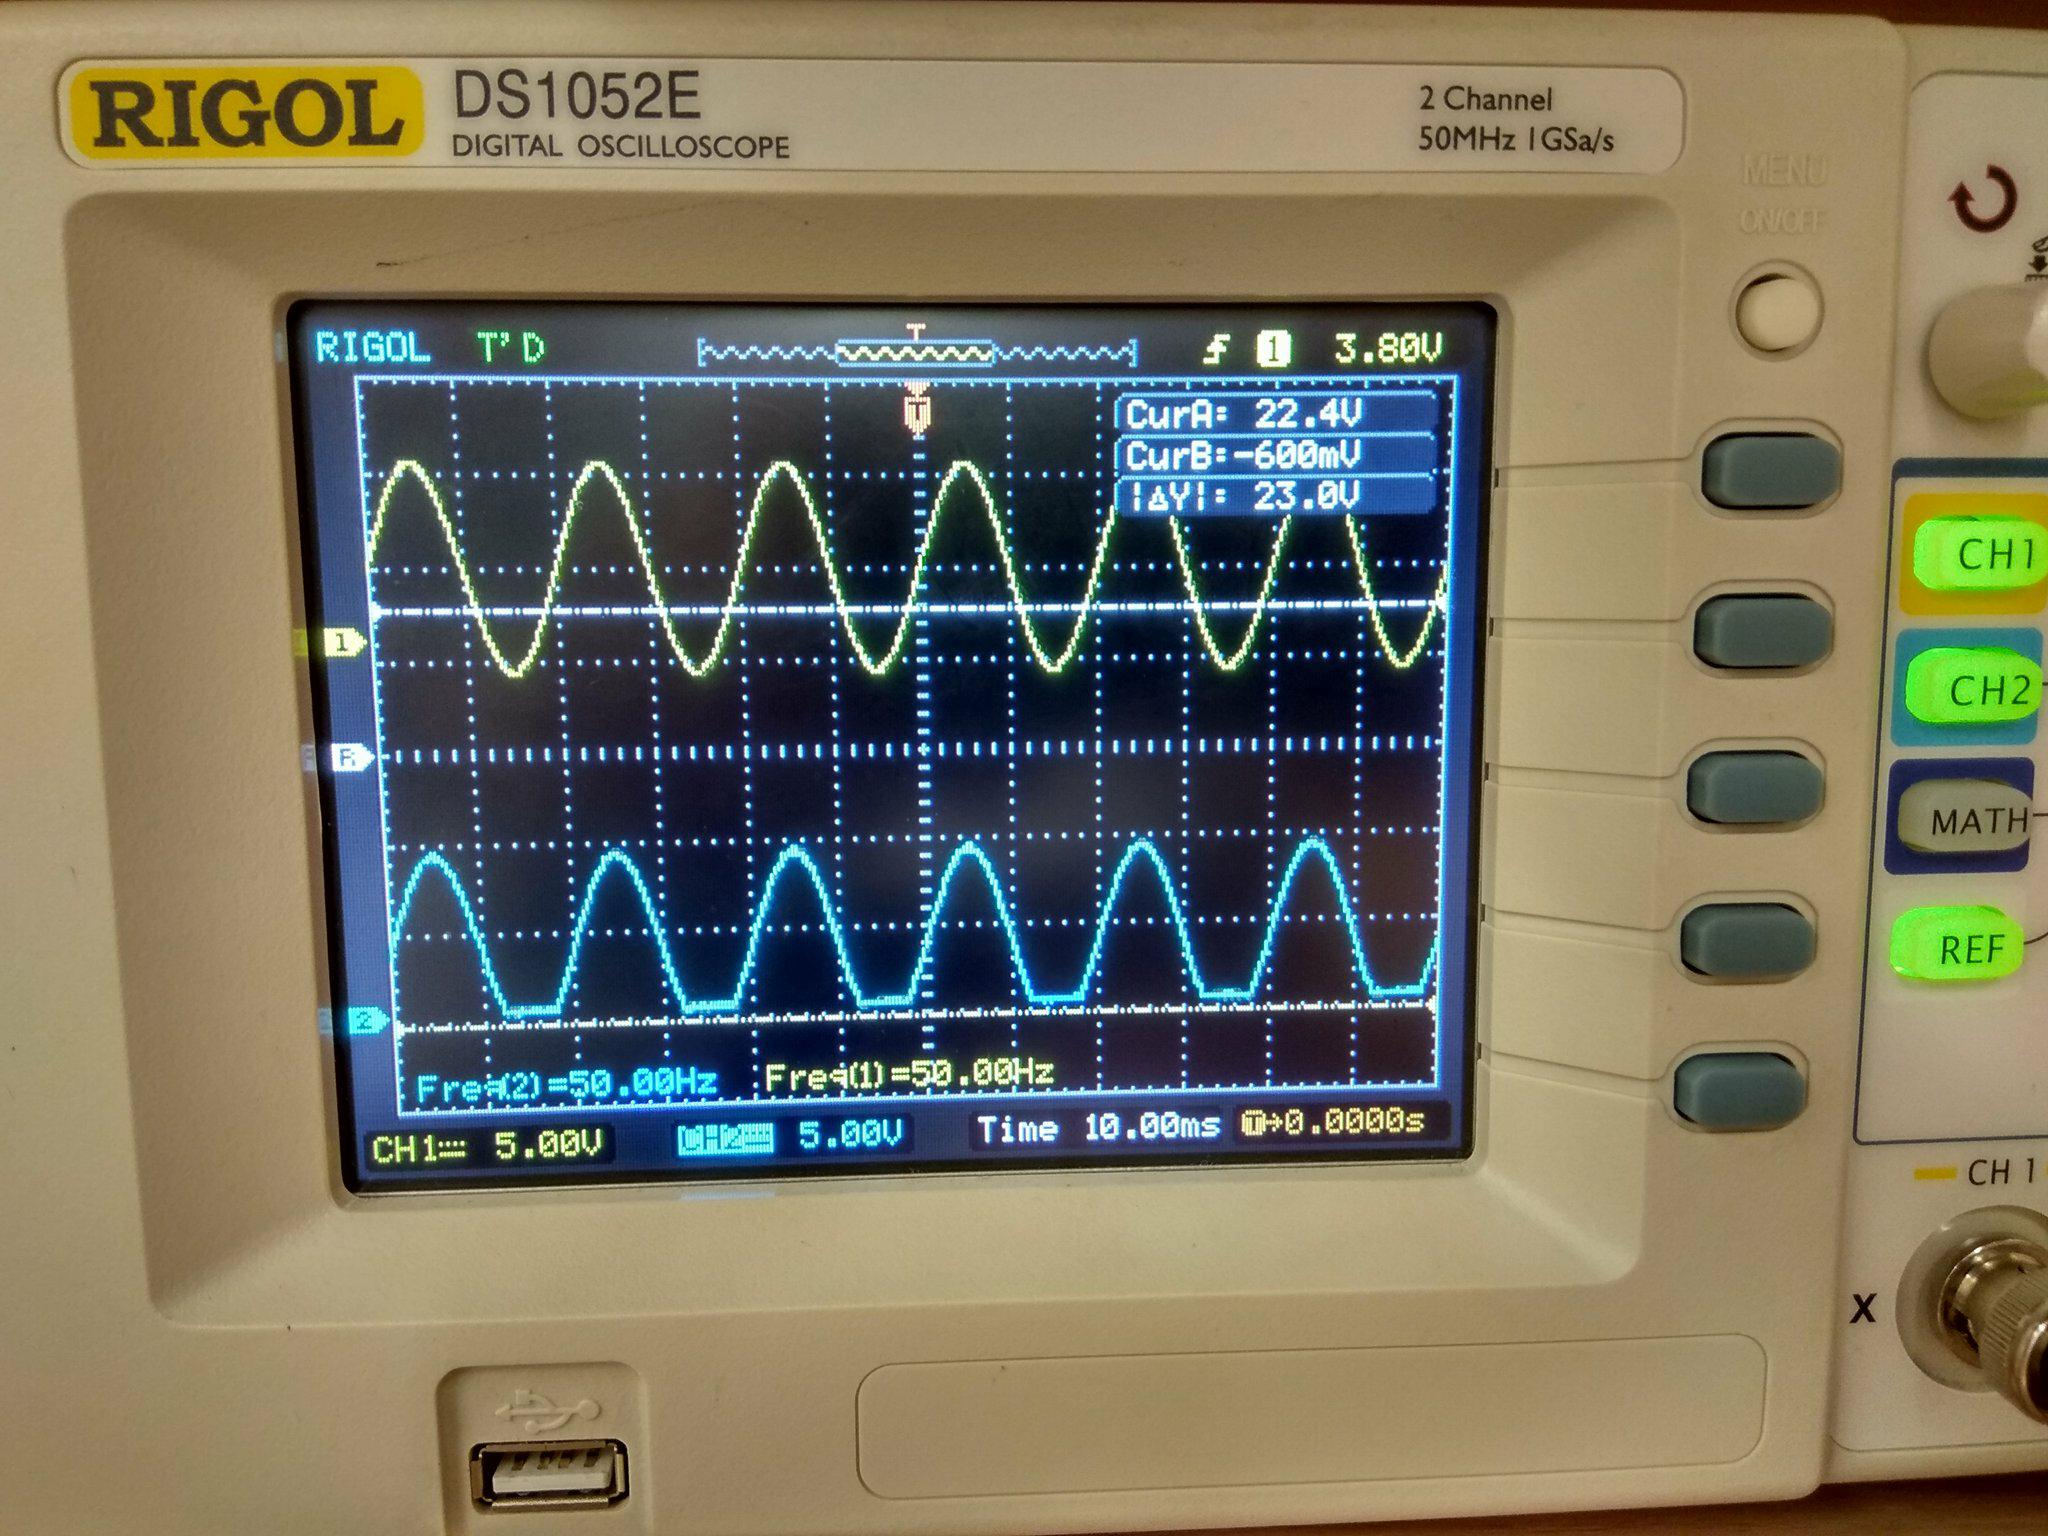
\includegraphics[scale=0.15]{2.jpg}
	\captionof{figure}{Oscylogram dla $R=200\Omega$ i $C_{f} = 2.2 \mu F$}
\end{figure}

\begin{figure}[H]
	\centering
	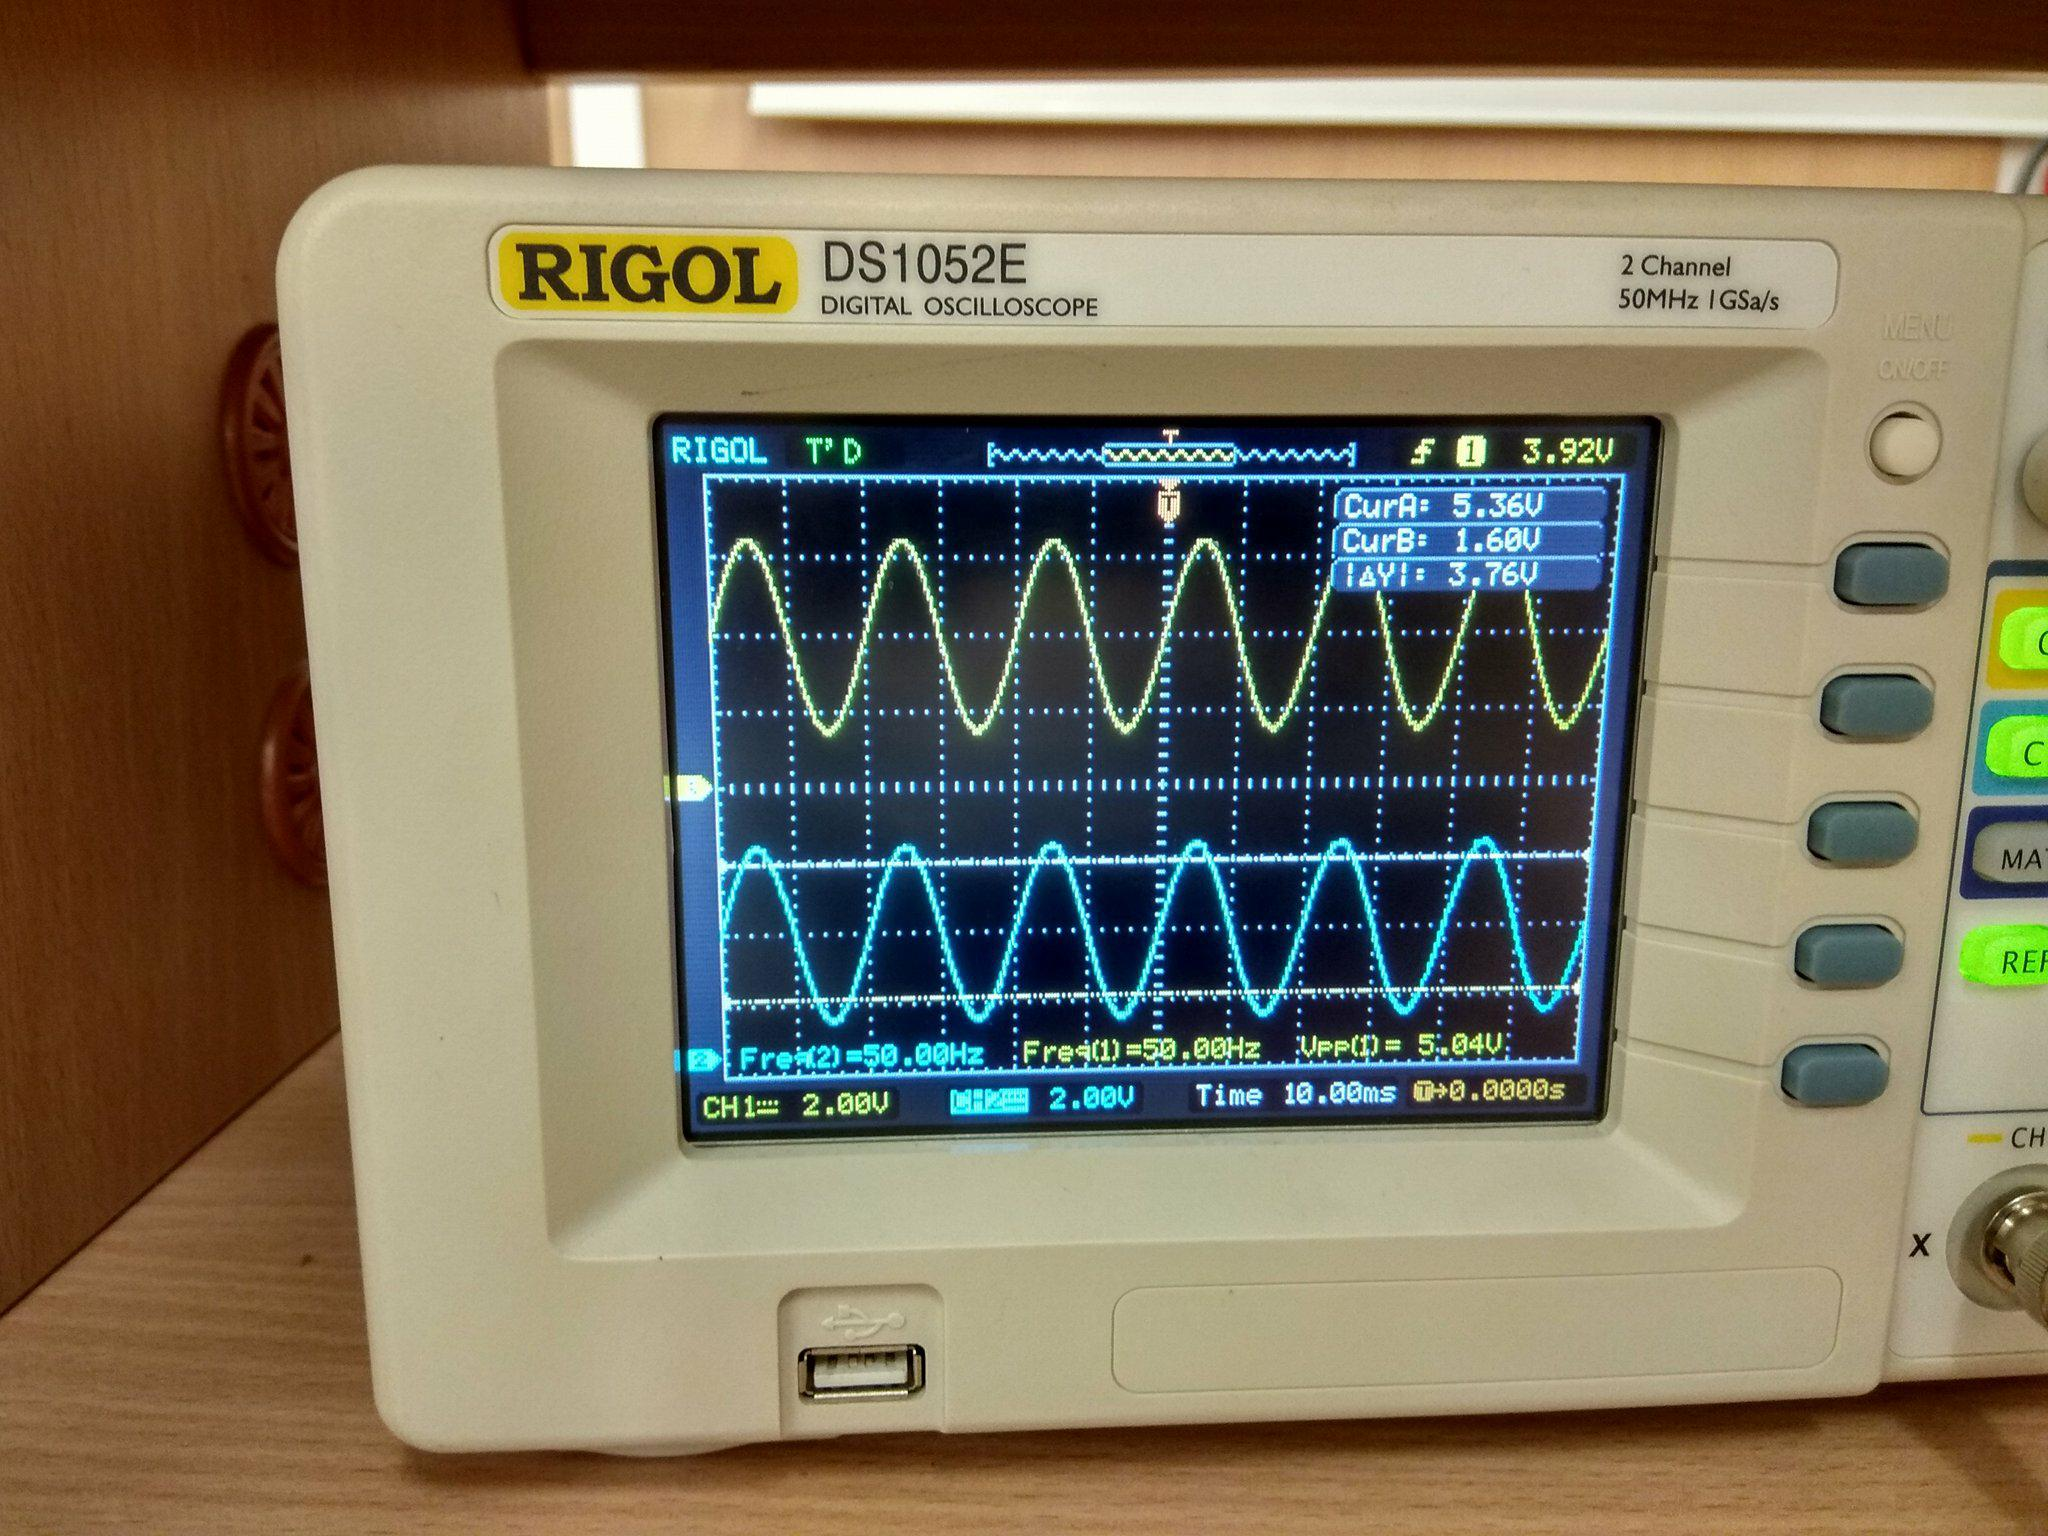
\includegraphics[scale=0.15]{3.jpg}
	\captionof{figure}{Oscylogram dla $R=2200\Omega$ i $C_{f} = 2.2 \mu F$}
\end{figure}

\begin{figure}[H]
	\centering
	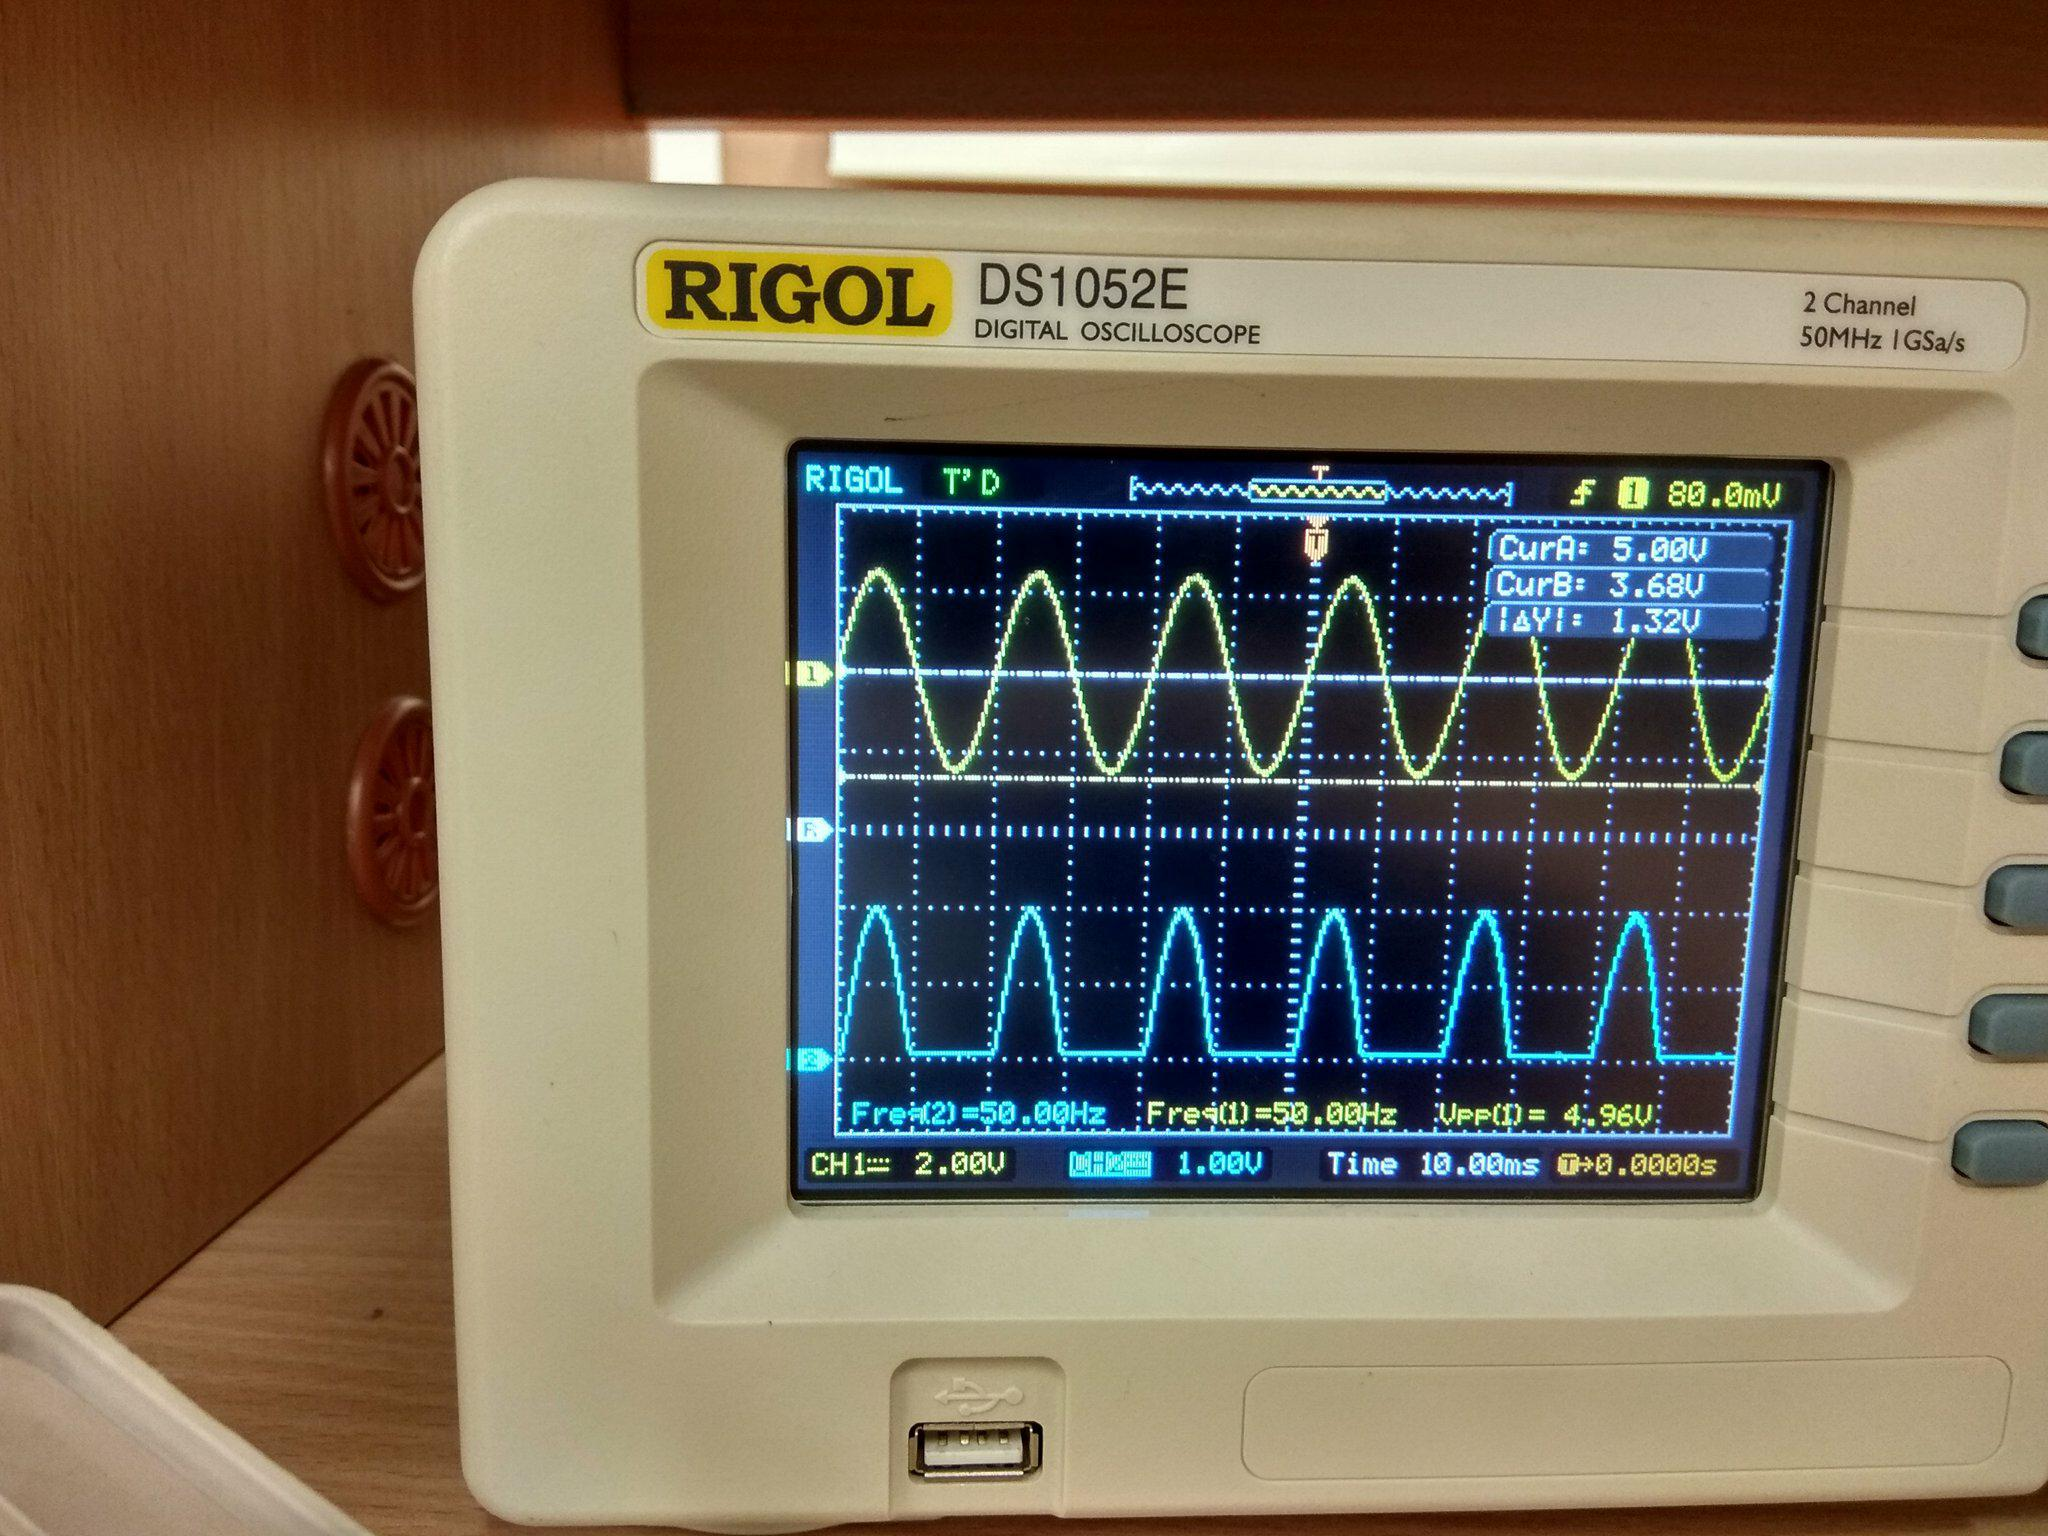
\includegraphics[scale=0.15]{4.jpg}
	\captionof{figure}{Oscylogram dla $R=2200\Omega$ i $C_{f} = 22 \mu F$}
\end{figure}

\begin{figure}[H]
	\centering
	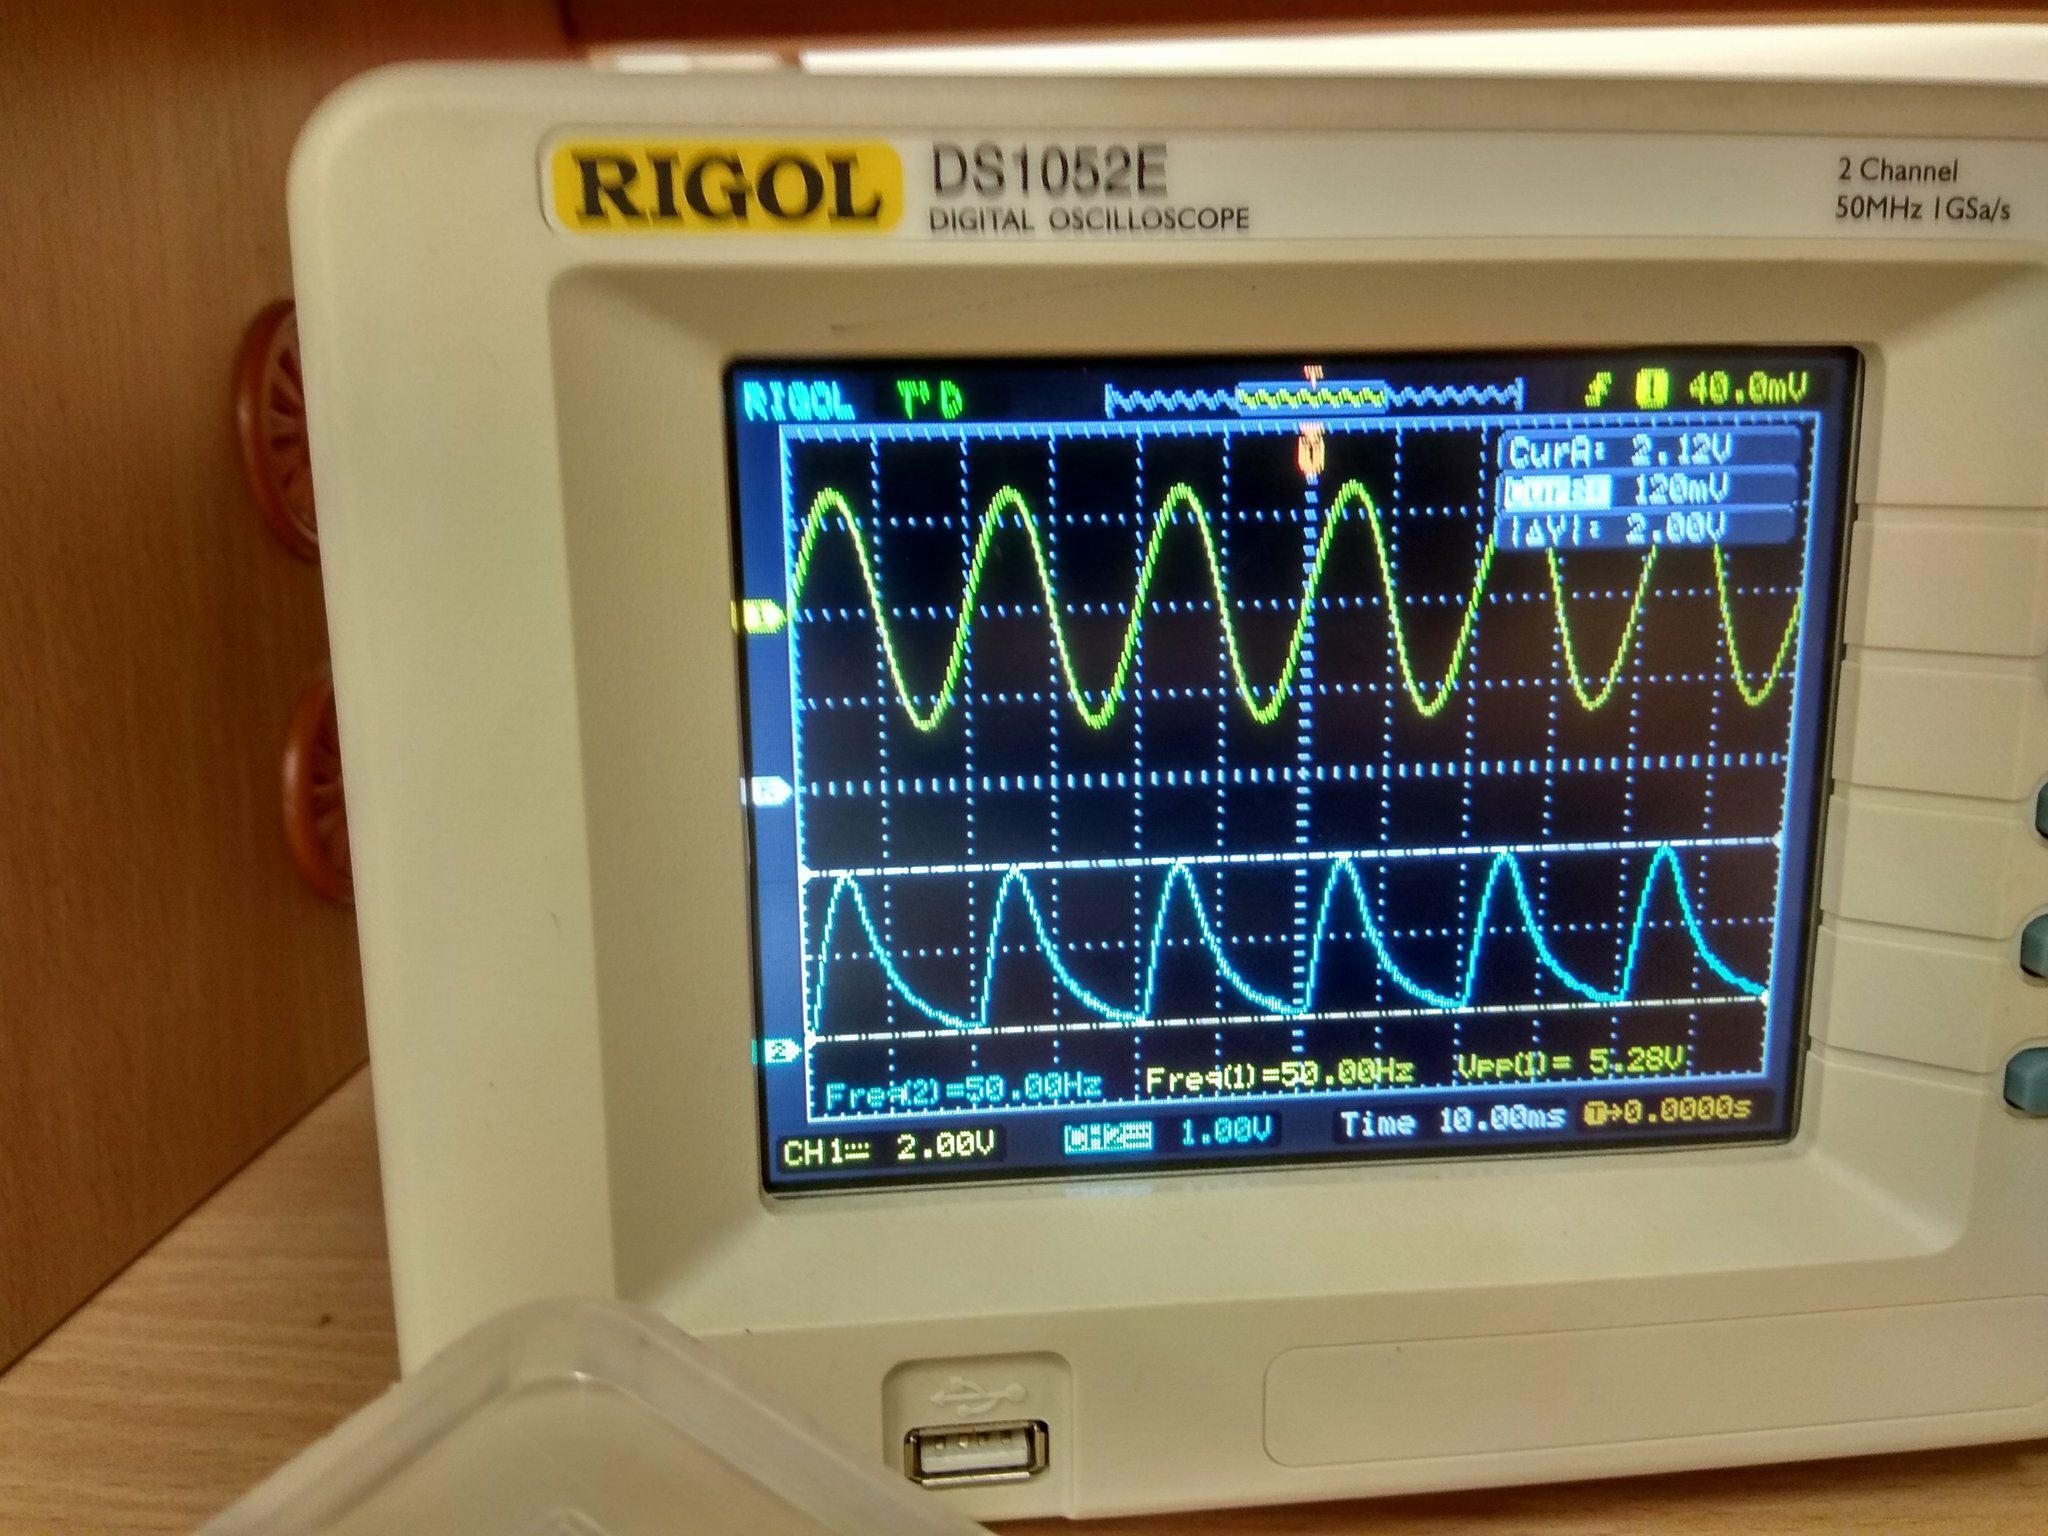
\includegraphics[scale=0.15]{5.jpg}
	\captionof{figure}{Oscylogram dla $R=200\Omega$ i $C_{f} = 22 \mu F$}
\end{figure}


\subsection{Wnioski}

Wraz z wzrostem pojemności filtrującej $C_{f}$ dla tych samych oporników, napięcie międzyszczytowe tętnień wzrasta. 


\section{Diody świecące}

\subsection{Cel zadania}

Badanie diod świecących.

\subsection{Przebieg zadania}

%%diody
\begin{figure}[H]
	\begin{equation*}
		\begin{circuitikz}
		\draw
		(0,0) to (4,0)
		to [european resistor, l=$R$, a=$1k\Omega$] (4,2)
		to (4,4)
		to[esource] (2,4)
		to[esource] (0,4)
		to (0,2)
		(0,0) to [american voltage source, l = $U_{in}$, a=$0..15V$] (0,2)
		(0,2) to[leDo] (2,2)
		to [leDo] (4,2)
		(2,2) to (2,4)
		(1,4) node[anchor = mid] {mV}
		(3,4) node[anchor = mid] {mV}
		(1,3) node[anchor = mid] {$D_{1}$}
		(3,3) node[anchor = mid] {$D_{2}$};
		\end{circuitikz}
	\end{equation*}
	\captionof{figure}{Schemat układu pomiarowego do badania diod świecących}
\end{figure}




\begin{figure}[H]
	\centering
	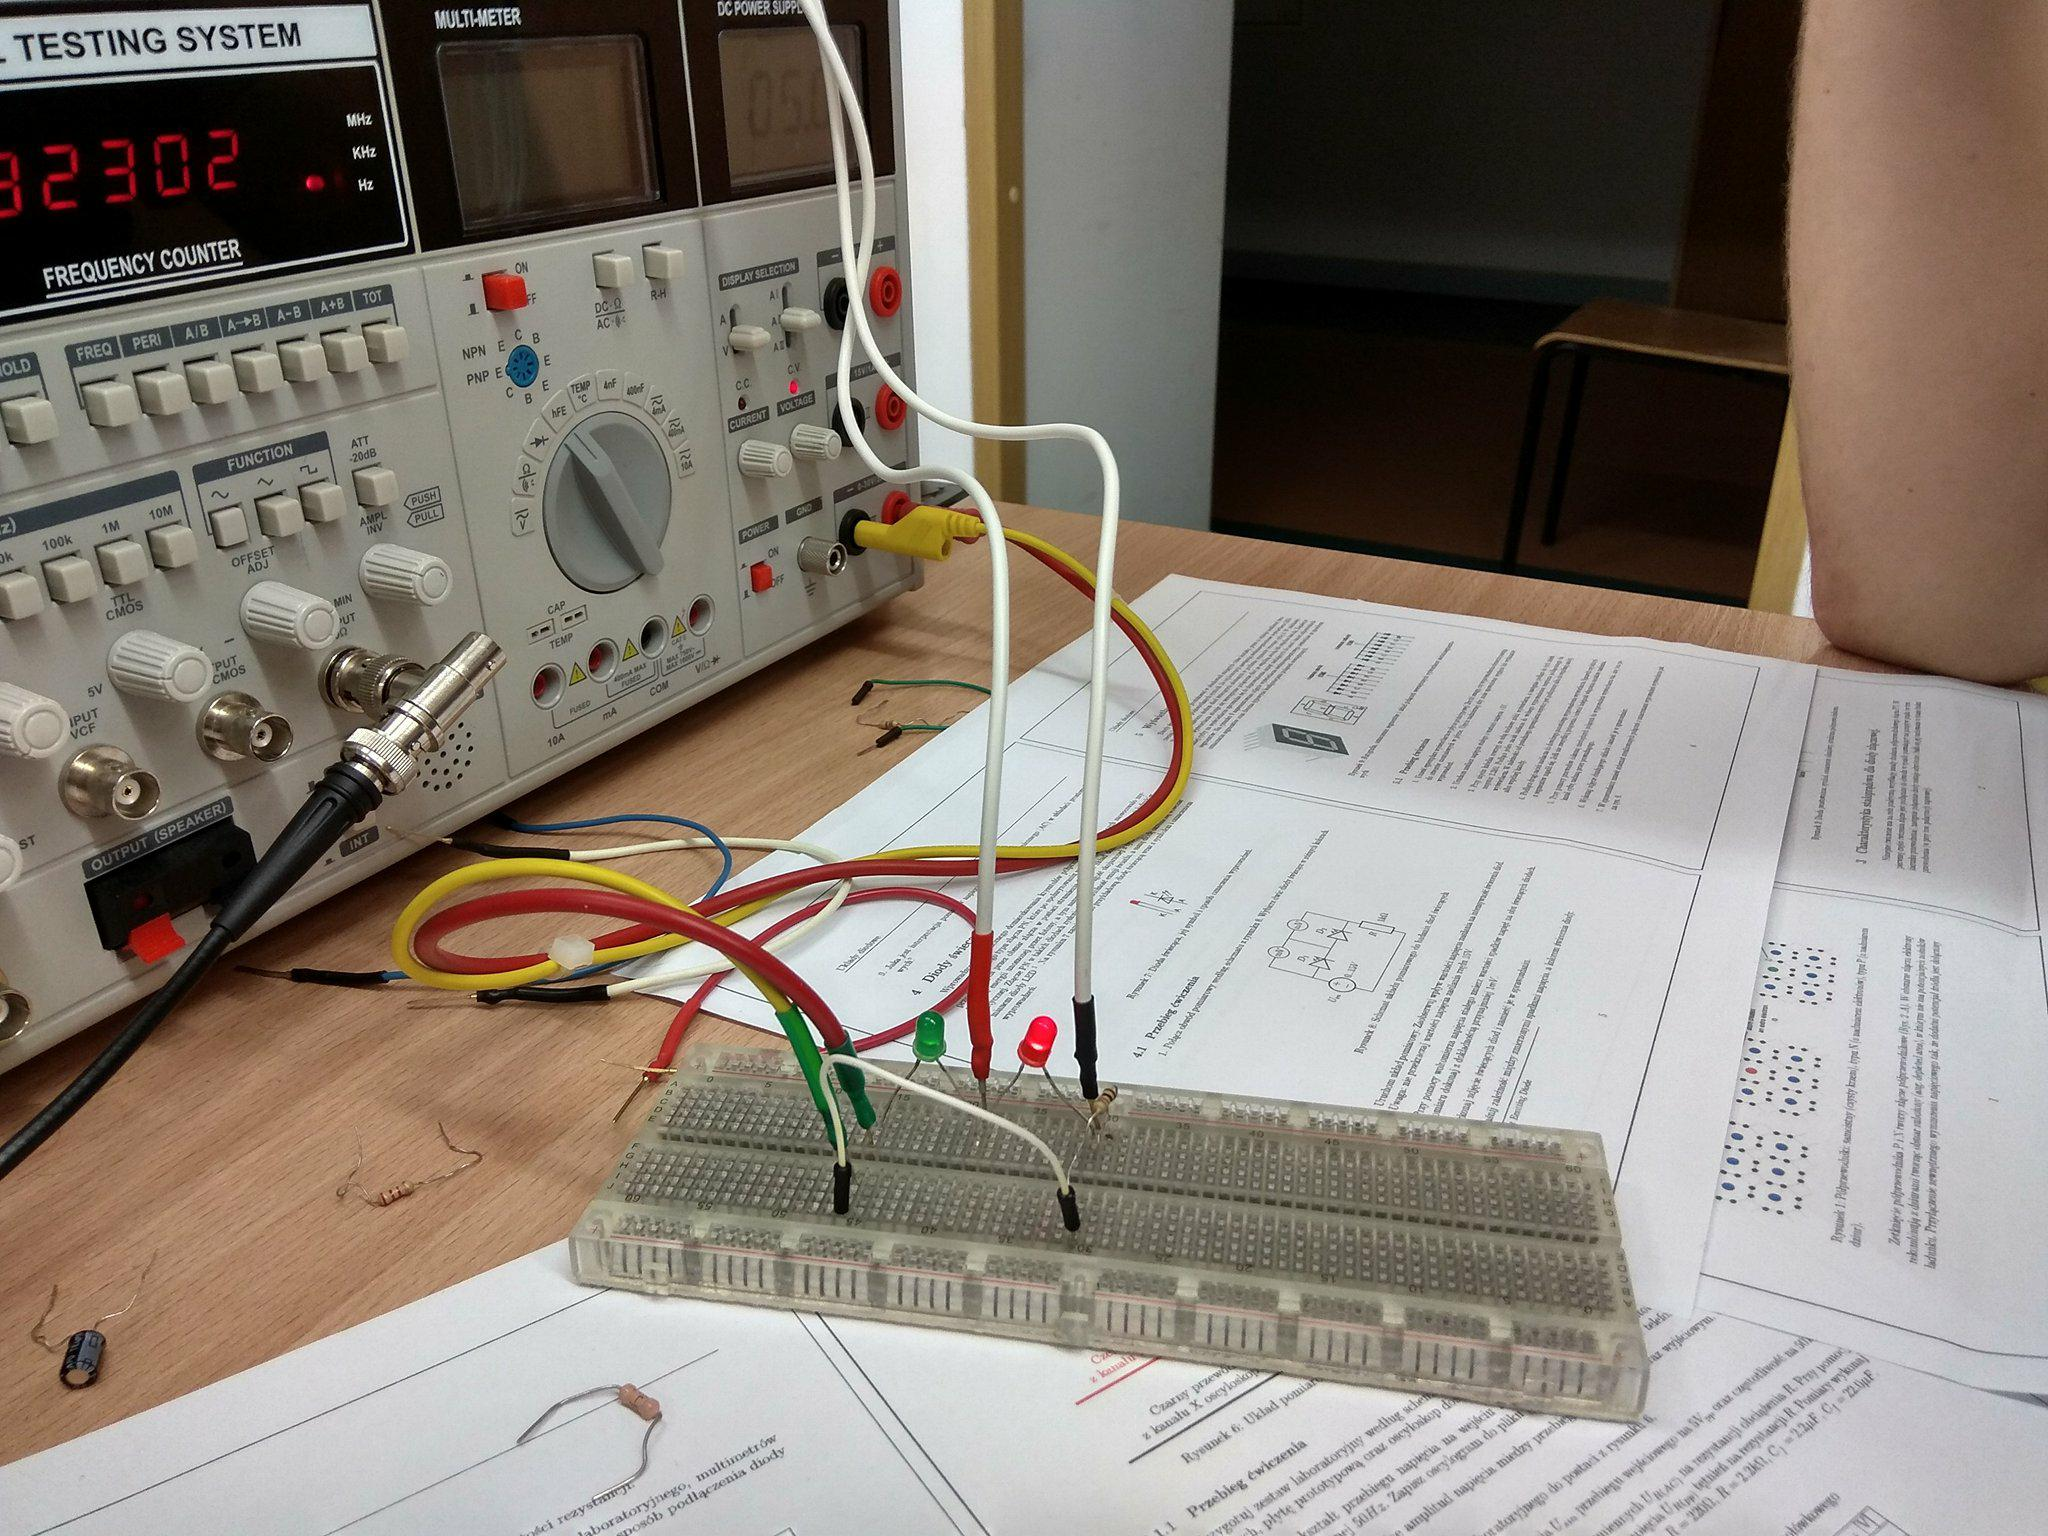
\includegraphics[scale=0.2]{5v.jpg}
	\captionof{figure}{Zdjęcie świecących diod przy napięciu zasilania $5V$}
\end{figure}

\begin{figure}[H]
	\centering
	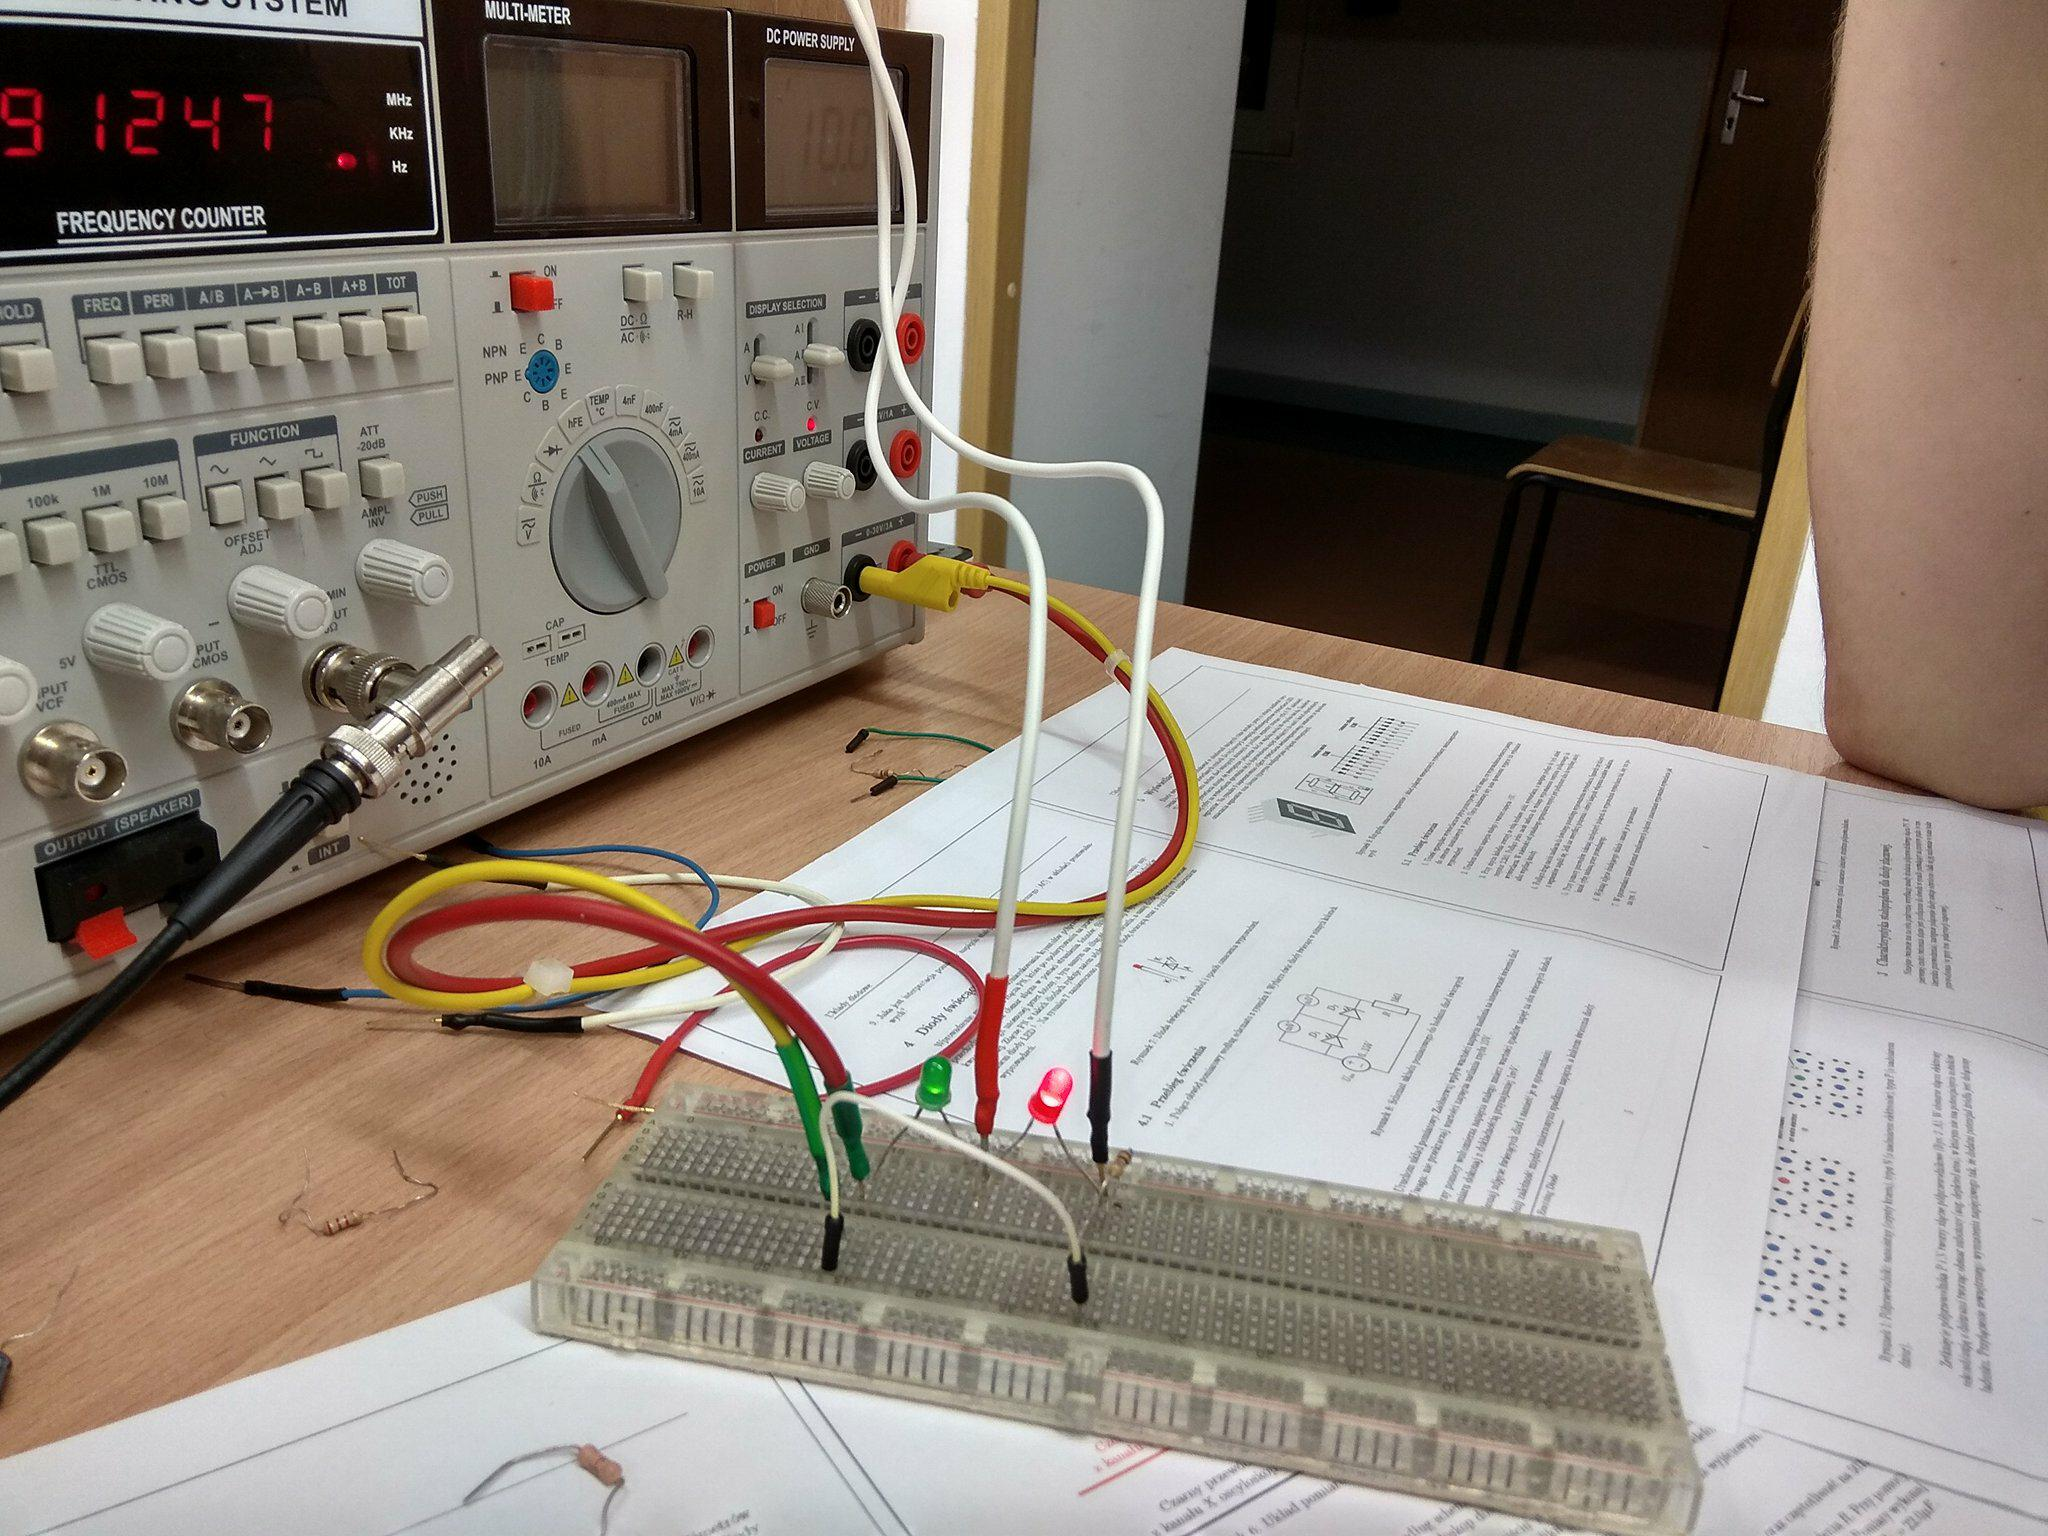
\includegraphics[scale=0.2]{10v.jpg}
	\captionof{figure}{Zdjęcie świecących diod przy napięciu zasilania $10V$}
\end{figure}

\begin{spacing}{1.5}
	\begin{equation*}
	\begin{array}{|r|r|r|}
	\hline
	\multicolumn{1}{|c|}{[V]}&\multicolumn{1}{c|}{D_{1}\quad[mV] \quad (green)}&\multicolumn{1}{c|}{D_{2}\quad[mV] \quad (red)}\\\hline
	5&2041&1724\\\hline
	10&2150&1846\\\hline
	\end{array}
	\end{equation*}
	\captionof{table}{Tabela prezentująca wyniki}
\end{spacing}

\subsection{Wnioski}

Wraz z wzrostem spadków napięć na diodach diody świecą jaśniej.

\section{Wyświetlacz LED}

\subsection{Cel zadania}

Badanie siedmosegmentowego wyświetlacza LED.

\subsection{Przebieg zadania}


\begin{figure}[H]
	\centering
	\includegraphics[scale=0.8]{nwm_bb.pdf}
	\captionof{figure}{Schemat zrealizowanych połączeń}	
\end{figure}

\begin{figure}[H]
	\centering
	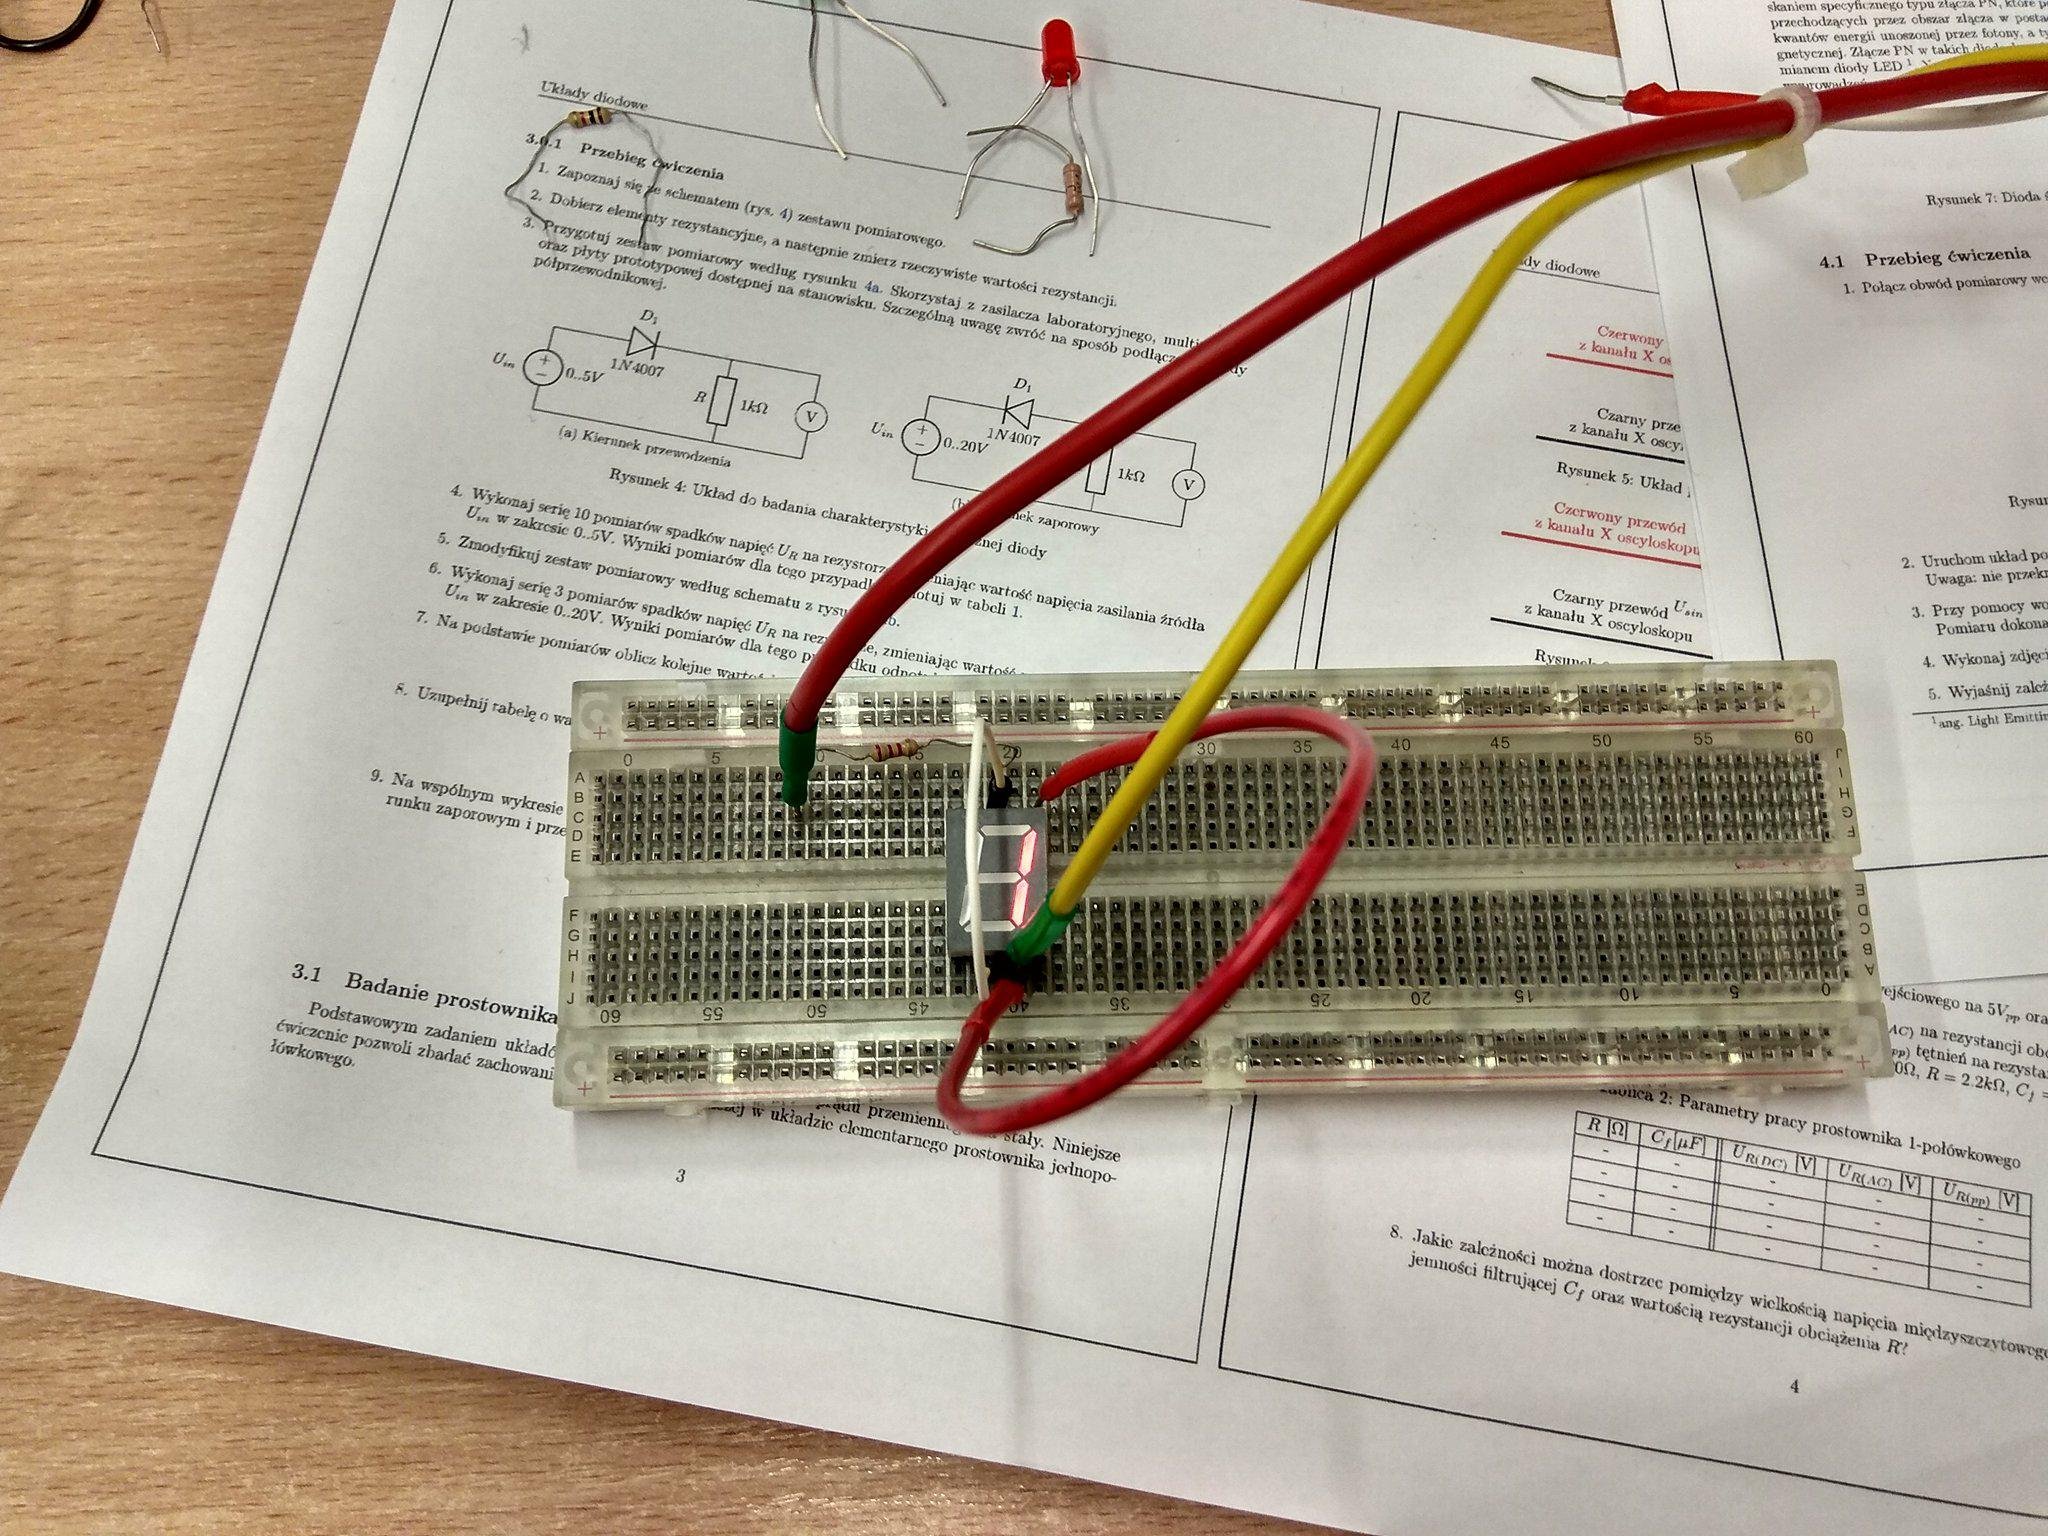
\includegraphics[scale=0.2]{display.jpg}
	\captionof{figure}{Na zdjęciu widać zdjęcie wyświetlacza 7-elementowego pokazującego cyfrę 1}
\end{figure}


	\begin{thebibliography}{99}
		\bibitem{pa}S. Bolkowski,  \emph{Teoria obwodów elektrycznych} , ser. Elektrotechnika teoretyczna. Wydawnictwa NaukowoTechniczne,
		1986, 
		\bibitem{pa1}P. Horowitz and W. Hill, \emph{Sztuka elektroniki}. WKiŁ, 2003, vol. 1.
		\bibitem{pa2}D. Halliday, R. Resnick, and J. Walker, \emph{Podstawy fizyki.} PWN, 2003, vol. 3.
		\bibitem{pa4}J. Watson,\emph{ Elektronika.} WKiŁ, 1999.
		\bibitem{pa5}Z. Nosal and J. Baranowski, \emph{Układy elektroniczne.} WNT, 2003.
	\end{thebibliography}
	\newpage
	\tableofcontents
		
\end{document}


